% Created 2026-07-09 Thu 08:41
% Intended LaTeX compiler: pdflatex
\documentclass{article}
\usepackage[utf8]{inputenc}
\usepackage[T1]{fontenc}
\usepackage{graphicx}
\usepackage{longtable}
\usepackage{wrapfig}
\usepackage{rotating}
\usepackage[normalem]{ulem}
\usepackage{amsmath}
\usepackage{amssymb}
\usepackage{capt-of}
\usepackage{hyperref}

\usepackage{fancyhdr}
\usepackage[top=25mm, left=25mm, right=25mm]{geometry}
\usepackage{longtable}
\fancyhead[R]{}
\setlength\headheight{43.0pt}
\usepackage[T1]{fontenc}
\usepackage[utf8]{inputenc}
\usepackage[spanish, ]{babel}
\usepackage[backend=biber]{biblatex}

\author{Leonardo Rodriguez, Henry Luisa, Evan Matango, Jonathan Pincay}
\date{2026-07-09}
\title{Booteo de Sistema Operativo Linux}
\hypersetup{
 pdfauthor={Leonardo Rodriguez, Henry Luisa, Evan Matango, Jonathan Pincay},
 pdftitle={Booteo de Sistema Operativo Linux},
 pdfkeywords={},
 pdfsubject={},
 pdfcreator={Emacs 27.1 (Org mode 9.7.5)}, 
 pdflang={Español}}
\begin{document}

\maketitle
\fancyhead[C]{
\includegraphics[scale=0.05]{images/logoEPN.jpg}\\
ESCUELA POLITÉCNICA NACIONAL\\FACULTAD DE INGENIERÍA DE SISTEMAS\\
ARQUITECTURA DE COMPUTADORES}
\thispagestyle{fancy}




\section{Objetivos}
\label{sec:orgb384172}

\begin{itemize}
\item Aprender a  bootear un sistema operativo Linux

\item Aprender sobre la secuencia de arranque de un computador como la
BIOS y la UEFI
\end{itemize}

\section{Instrucciones}
\label{sec:orgc4129b1}
\begin{enumerate}
\item Siga el tutorial para la creación de un booteable de Ubuntu como se
indica en la unidad 9 en el archivo Arranque Ubuntu\footnote{Dependiendo de las características de su computador debe
verificar si al crear el medio booteable para Ubuntu, su sistema
reconoce o acepta para el \emph{Target System}}.

\item Realice un respaldo del código de \emph{BitLocker} utilizando un command
prompt de Windows con permisos de administrador\footnote{Si no respalda el código, no podrá arrancar el disco luego de
reiniciar. Más información en: \href{https://www.partitionwizard.com/disk-recovery/bitlocker-recovery-key-bypass.html }{https://www.partitionwizard.com/disk-recovery/bitlocker-recovery-key-bypass.html}}:

\begin{verbatim}
    manage-bde-protectors C:-get
\end{verbatim}

\item Utilizando su computador o el del laboratorio, siga los pasos
indicados para obtener el booteo desde el USB con el Sistema
Operativo de Ubuntu

\item Realice el boot de Ubuntu desde la memoria USB externa y
seleccione la opción de \emph{Probar Sistema Operativo}.
\item Una vez ingresado active un terminal de Ubuntu: \texttt{Ctrl+ALT+T} y
obtenga las características del computador mediante la ejecución de
los comandos: \texttt{lscpu}, \texttt{lsb\_release -a} y \texttt{lspci}. Obtenga capturas
de la ejecución de los comandos. Luego abra este archivo en WSL y
ejecute los comandos desde los bloques shell. Para insertar un
bloque puede usar la combinación \texttt{C-c C-,}, escoja la opción \texttt{src}
e indique que es del tipo shell.
\end{enumerate}

\section{Desarrollo Emacs}
\label{sec:orgb629418}
Se sugiere utilizar la opción \texttt{:fontsize
scriptsize} para dar formato a la ejecución del comando. Por ejemplo,
considere:

\begin{verbatim}
whoami
\end{verbatim}

\begin{verbatim}
leningfe
\end{verbatim}

\subsection{Comando \texttt{lsb\_release}}
\label{sec:org3032273}
\begin{verbatim}
    lsb_release -a
\end{verbatim}


\subsection{Comando \texttt{lspci}}
\label{sec:org54ab2b8}
\begin{verbatim}
    lspci
\end{verbatim}


\subsection{Comando \texttt{lscpu}}
\label{sec:org734fb50}
\begin{verbatim}
    lscpu
\end{verbatim}

\section{Desarrollo Capturas}
\label{sec:org21fc0f8}
Coloque las capturas de los resultados obtenidos en los
terminales. Para esto recuerde utilizar dobles corchetes y escribir el
\emph{path} hacia la imagen. Pruebe a utilizar YASnipet para generar el
siguiente código para descripción de la figura. Para esto puede
escriba \texttt{fig\_} seguido de la combinación de teclas \texttt{C-TAB}, finalmente
coloque la dirección de la imagen.

\begin{figure}[htbp]
\centering
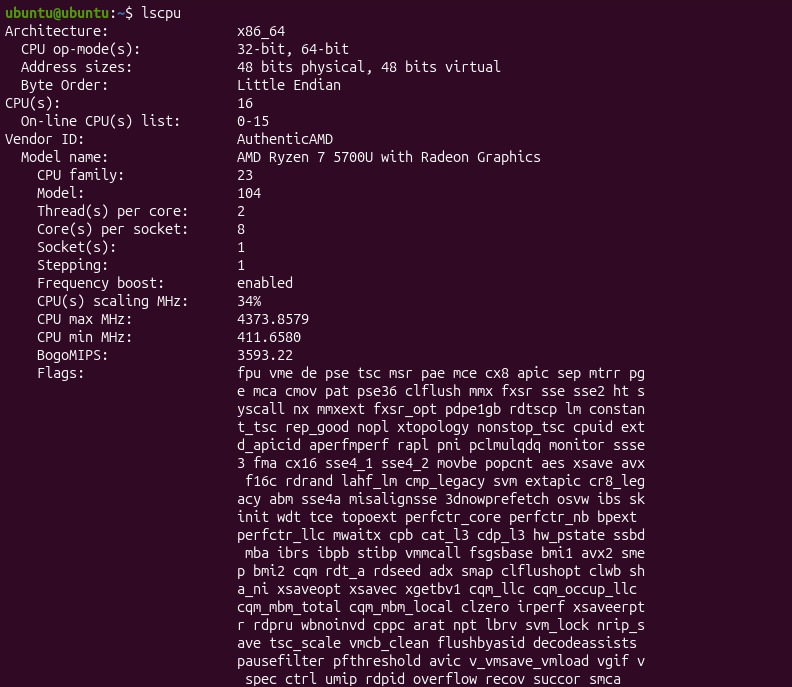
\includegraphics[width=0.85\textwidth]{images/lscpu.jpeg}
\caption{Ejecución del comando lscpu (Parte 1)}
\end{figure}

\begin{figure}[htbp]
\centering
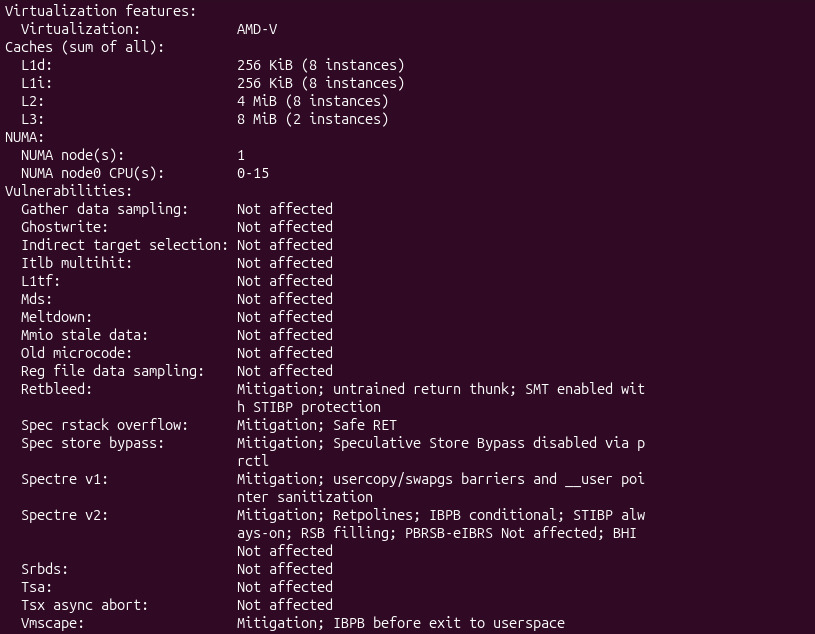
\includegraphics[width=0.85\textwidth]{images/lscpu2.jpeg}
\caption{Ejecución del comando lscpu (Parte 2)}
\end{figure}

\begin{figure}[htbp]
\centering
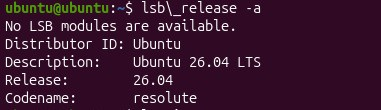
\includegraphics[width=.9\linewidth]{images/lsb.jpeg}
\caption{\label{fig:org0fbaf57}Ejecución del comando lsb\textsubscript{release} -a}
\end{figure}

\begin{figure}[htbp]
\centering
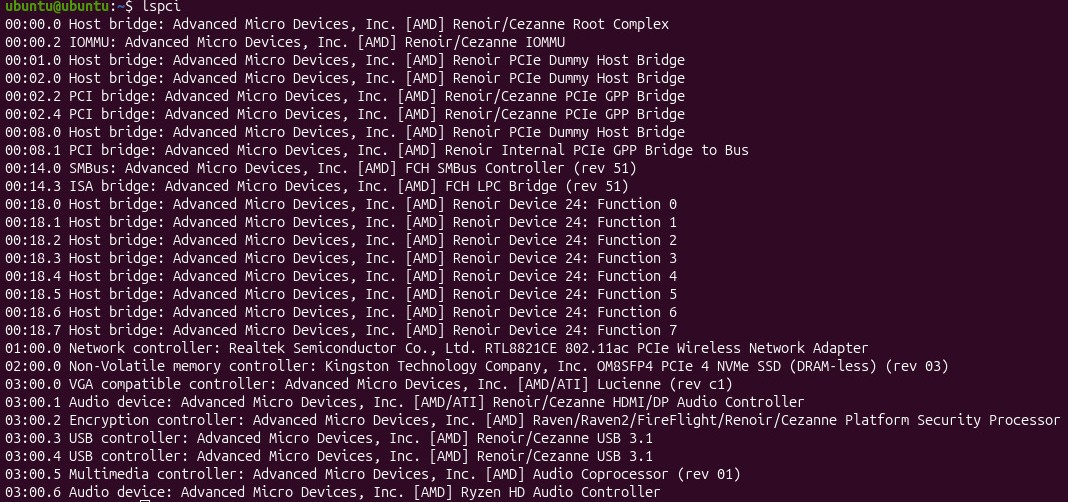
\includegraphics[width=.9\linewidth]{images/lspci.jpeg}
\caption{\label{fig:orge56a071}Ejecución del comando lspci}
\end{figure}

\section{Consulta}
\label{sec:org048afd6}
Describa que hacen y para qué sirven los comandos utilizados en la práctica

\begin{description}
\item[{lscpu}] 
\end{description}
Sirve para mostrar información detallada sobre la arquitectura de la
CPU (el procesador) de tu computadora.  En lugar de tener que revisar
archivos complejos del sistema, lscpu reúne esos datos y los presenta
en la terminal de una forma limpia, organizada y fácil de
leer.

\begin{description}
\item[{lsb$\backslash$\textsubscript{release} -a}] 
\end{description}
Sirve para mostrar información sobre la distribución de Linux que
tienes instalada. 

\begin{description}
\item[{lspci}] 
\end{description}
El comando lspci es una herramienta de diagnóstico fundamental en
sistemas Linux. Sirve para listar todos los dispositivos de hardware
que están conectados a la placa base de tu equipo a través de los
buses PCI (Peripheral Component Interconnect).
\end{document}
